\chapter{System design}

In this chapter the previously collected information is used to design the system in detail.
The decision making process for that is documented here as well.

%\todo{mention? decentralization aspects?}

\section{Environment}

All Winslow instances are supposed to run inside a Docker container (as requested in \autoref{workflow:desired:docker}).
The hosts will be Ubuntu or Debian Linux Servers of which some will have one or multiple GPUs.
There will be no graphical user interface available on these servers.

The decision to implement Winslow in Java was made early on.
This has three main reasons, first, the developer is experience in Java development, the server side web framework used is a Java library (see \autoref{design:springboot}) and the company this implementation is for has a focus on Java development.
This means if the system is successful, maintenance and possible extensions might be authored by another developer who has probably knowledge in Java development as well.
% \todo{.cleanup}

%\todo{env: shall be executed on ubuntu/debian linux servers, Docker}

\section{Storage Technology}

Organizing and accessing data is one of the main concerns for Winslow.
In almost all use cases, multiple instances will need to access the storage.
It must therefore be accessible from remote and by multiple Winslow instances simultaneously.
For that, the following technologies are reviewed: NFS or SMB/CIFS (\autoref{analysis:storage:organisation}),  GlusterFS (\autoref{glusterfs}), SeaweedFS (\autoref{seaweedfs}), OpenIO (\autoref{openio}), dCache (\autoref{dcache}) and HadoopFS (\autoref{hadoopfs}).

The following criteria were used for comparison.
The scoring system provides points from 0 to 3, in which 0 means the best solution and 3 the worst.
The points of the individual categories are added together, the lowest overall score shall then point to the best solution:

\begin{itemize}
\item \textbf{Installation Overhead}:
How hard and extensive is the installation?
Is there a good documentation?
Is the package provided from within the main repository of Ubuntu, Debian, or alternatively, does it provide any other form of easy installation?
Scoring 0 for installation through the main repository, 1 for an external repository, 2 for a distribution specific archive, 3 for any other installation solution.

\item \textbf{Dependencies}:
Are further services required for operation? 
How hard are they to setup?
Do they need any additional configuration?
Scoring 0 for no further dependencies, 1 for dependency requirements but without the need of manual configuration,  2 for dependencies that require manual configuration, 3 for dependencies that need to be installed manually and require manual configuration.

\item \textbf{Single Point of Failure}:
Is the solution decentralized and is it failure resilient?
Is it site- or rack-aware or provide replication mechanisms to compensate?
Scoring 0 for completely decentralized, 1 for no direct SPoF but with a dependency on a centralized backend, 2 for a mostly centralized solution but with load balancing approaches, 3 for no single point of failure mitigations.

\item \textbf{Docker integration}:
How easy is it to integrate with Docker?
Scoring 0 for native support, 1 for native but non-trivial support, 2 for support through additional exports facility, 3 for non-trivial solution.

\item \textbf{Failure concerns}:
Are there any noteworthy concerns?
Was an early local test successful and reliable?
Is it a known technology or \enquote{proven in use}?
Who is developing it and what are the support guarantees?
Scoring 0 for commonly used and no concerns, 1 for minor concerns, 2 for major uncertainty, 3 for abandoned technology.
\end{itemize}

In \autoref{comparision:storage} the results are displayed:

\begin{table}[H]
	\begin{tabular}{|l|c|c|c|c|c|c|}\hline
				& NFS S.& SMB/CIFS S.& GlusterFS & SeaweedFs	& dCache 	& HDFS \\
		\hline
		Inst. 	& 0 	& 1 		& 0 		& 2 		& 3			& 1 \\
		Dep. 	& 1 	& 0			& 0 		& 0 		& 3 		& 1 \\
		SPoF 	& 2		& 3			& 0			& 2 		& 0			& 0 \\
		Docker 	& 0 	& 2 		& 2 		& 3 		& 2 		& 3 \\
		Fail.	& 0		& 0			& 1			& 2			& 2			& 0 \\
		\hline \hline
		Score 	& 3		& 6			& 3			& 9			& 10		& 5 \\ \hline
	\end{tabular}
	\caption{Failure concern comparison of storage technologies}
	\label{comparision:storage}
\end{table}

The worst scoring tool in this comparison is dCache.
The installation overhead, missing documentation and uncertainty on reliable operation is too high for this project (see \autoref{dcache}).

For similar reasons SeaweedFs is placed second worst.
Local tests could not access SeaweedFs reliable when a node failed and there is no trivial support for Docker nor does it provide an NFS export.
Using it would require each started container to be manipulated so that the first operation is mounting the storage with a custom binary and through a FUSE\footnote{Filesystem in Userspace} mount.
The tool also seems to be developed by a single person which introduces further uncertainty about reliability and support in the future.

HDFS and SMB/CIFS seem to be no terrible choice, but no especially good one either in this use case.

The two best scoring storage solutions are a simple NFS share and GlusterFS.
While GlusterFS provides replication and decentralized access, a NFS share scores with its simplicity.
The idea is to start with a plain NFS share for Winslow which can natively be utilized by Docker as volume mount and to revisit later whether the need for replication and decentralization persists.
Because of the NFS export feature of GlusterFS, Winslow could then easily switch to GlusterFS.



\section{Execution Management}

As noted in \autoref{analysis:layer_1}, the central business logic is to decide on when and to issue stage executions.
Generally speaking, there are two approaches when executing jobs: local or remote. Both will be discussed next.

In the remote approach, the job is executed on a machine that is not the same that has the responsibility to manage the process.
Continuous Integration (CI) platform Jenkins\cite{jenkins:main} does use this approach.
A so called slave node (Jenkins) is contacted through a native interface (SSH for Linux servers) to transfer resources and to start the job process.
In this scenario, the CI instance requires and stores login credentials for every remote machine to be able to login whenever needed.
The system administrator has to create a new user accounts on the remote machines, install required programs and prepare the environments.
One big risk for this approach is that in case of any security breach on the central CI instance, the attacker is also able to login on all remote machines.

GitLab\cite{gitlab:main} follows a more local approach, where the system administrator has to manually install the GitLab Runner on machines that are then able to connect to GitLab and execute jobs.
This runner is responsible in pulling jobs, executing them locally, monitoring and reporting back the outcome.

Winslow is going to follow the local approach.
On each physical machine that is supposed to provide compute resources, Winslow needs to be installed.
The installation is expected to be easy, as is based on starting a prepared Docker image.
An election between the Winslow instances is selecting the most fitting hardware for a stage execution (see affinity and aversion in \autoref{election:affinity_and_aversion}).
It is expected that each instance can judge this best on its own, as it knows which resources are available.
Work is distributed to an executor as it is detected.



\section{Event Synchronization and Communication}
\label{design:synchronization}

\begin{comment}
kafka does what? persist events and provides them in an order(?), cant Winslow do this itself, so that no further dependency is required?

\todo{.}
https://docs.microsoft.com/de-de/azure/architecture/microservices/design/interservice-communication


raw TCP (how to connect, centralized? star? tree?) centralized works towards -> centralized master node
broadcast?
microservice REST
event bus? kafka
messaging queue mqtt
NFS provides filesystem, filesystems are kind of standardized

https://kafka.apache.org/protocol
\todo{.}
\end{comment}


As discovered in \autoref{analysis:layer_2}, there is the need for event synchronization across all Winslow instances.
Without proper coordination, race conditions could cause stages to be started multiple times simultaneously, corrupt workspaces, configuration or project files.
While starting too many stage executions are only wasting resources, data corruptions can lead to unrecoverable damage.

There are multiple ways to exchange data between systems that do not share the same process or machine.
The most flexible implementation can be achieved by implementing a custom protocol on a raw TCP socket which allows to exchange blobs (Binary Large Objects) between exactly two nodes.
For a blob or message to reach all nodes, a connection to every other node, a centralized broker, another topology such as a tree structure or broadcast messages would be required.
Because this in itself seems to be a complex subject, third party alternatives were investigated.

Apache Kafka\cite{kafka} is one such alternative.
It is open source, distributed and is focused on providing a system wide ordered data and event stream that can be persisted over a certain time period.
But as every third party service, it introduces a dependency on the project.
Not only in regards to interfacing and driver implementation, but also for maintenance and setup.
Each Winslow Image would require to be shipped with a pre-configured Kafka service and the administrator must ensure that these services can reach each other - in addition to the storage solution.

Instead, it would be quite elegant, if an already planned connection between all Winslow instances could be reused for this, which could eliminate the need for third party dependencies here.
For now, only a common storage is required.
Re-using this as communication channel, a mechanism must be found to give each occurring event a sequence number, that is unique system wide.
New events would not be allowed to be propagated by an instance before it processed all previous events.
With this idea in mind, messages that can be used coordinated all required actions are defined next.

\begin{comment}

\todo{ACID in fundamentals?}
ACID, which stands for Atomicity, Consistency, Isolation and Durability, describes the needs a database must fulfill so that it does not suffer from side effects or data corruption when executing queries.
A series of changes might not be allowed to be intercepted (atomicity), must see and result in consistent data, is not allowed to interfere with simultaneously executed queries and guarantees that once completed successfully, is in fact persistent and will not be lost (durability).

\todo{filesystem is close}

\todo{DB principles: ACID}

\todo{...}

\todo{requires common a way to exchange messages}

\todo{all messages - called events - are published to all nodes}

\todo{using file system as bus}

\todo{clear and globally same order of events}

\todo{events consist of an id, command, time, duration, subject and issuer}

\todo{events might have a duration}

\todo{unspoken requirement: all nodes share the same clock - or one with very little drift}

\todo{usage as synchronization primitive}
\end{comment}

\subsection{Messages}
\label{message:grace_period}

To coordinate the Winslow instances, the messages will be exchanged through the common event bus, which broadcasts every message to all instances.

Because this is a multi instance system which can suffer partial failure, all multi-part operations have to have a timeout attached, so that a failure is detectable.
Without this timeout, one could not detect the absence of a finish signal for a multi-part operation, which could potentially block further operations for forever.

To account for transmission delay and slight clock offsets an additional time padding is granted.
Because of the non-requirement for real-time scheduling this can generously be set to 5 seconds.

All exchanged messages must share a common structure, which is listed next:

\begin{itemize}
	\item \textbf{issuer}: The id of the Winslow instance that published the message
	\item \textbf{command}: The state change request (described a bit further below)
	\item \textbf{subject}: What the command is about to change
	\item \textbf{timestamp}: The time of when the message was issued
	\item \textbf{duration}: Optionally, a non zero time period of the expected duration
\end{itemize}

With this message structure definition, the following commands can be used:

\begin{itemize}
	\item \textbf{LOCK}: Locking a resource, commonly a project.
	A lock is exclusive to the issuer and can only one at a time can be granted for a subject.
	\item \label{message:extend} \textbf{EXTEND}: Updating an ongoing operation by extending the timeout.
	This can be used to signal that a lock is still required although its timeout is about to be reached.
	The duration of the original event is extended and therefore the timeout is pushed back.
	The issuer must be the same as the issuer of the operation that is referred to.
	\item \textbf{RELEASE}: Releasing a locked resource.
	The issuer must be the same node as the one that issued the \textbf{LOCK} previously.
	\item \textbf{KILL}: Non-gracefully stop an operation or destruction of a lock.
	This signals that an operation shall be stopped or that the lock shall be released immediately.
	This can be used to abort an running stage execution.
	\item \textbf{ELECTION\_START}: Signals that an election for a stage execution has started.
	The signal must refer to an project that can make progress.
	\item \textbf{ELECTION\_PARTICIPATE}: Signals that the issuer node is capable of executing the next stage of the mentioned project.
	It also includes a scoring for the affinity and aversion (more details in \autoref{election:affinity_and_aversion}).
	This message must always refer to a valid election.
	\item \textbf{ELECTION\_STOP}: Signals that an election has finished.
	The participator with the best score is now allowed execute the next stage of the referred project.
	This is signal is only allowed to be issued by the same node that started the election process.
\end{itemize}

\subsection{Synchronization}

In a file system two files with the same name are not allowed to exist in the same directory, which is ensured by the filesystem.
This can be used when publishing events in a common directory: a by all instances followed sequence number is used as file name.
Publishing a new event will fail, if there already exists a file for that sequence number.
Watching the directory will then also result in a stream of ordered events.

To publish an event, a naive implementation would first check the directory for the next number in the sequence and to create it, if it was not found.
But this has a potential race condition: between checking for the file and creating it, another instance could have created the file.
Luckily, the POSIX standard provides a flag when creating files, that will expose this conflict by returning an error, if \enquote{Both O\_CREAT and O\_EXCL are set, and the named file already exists}\cite{gnu:open}.
This mechanism is also exposed in Java by calling \javacinline{Files.write(..)}\cite{javadoc:files:write} with \javacinline{StandardOpenOptions.CREATE\_NEW}\cite{javadoc:standard_open_options:create_new}.
The behaviour of publishing an event can therefore be summarized with \autoref{event:synchronized_publish}:

\begin{figure}[H]
	\centering
	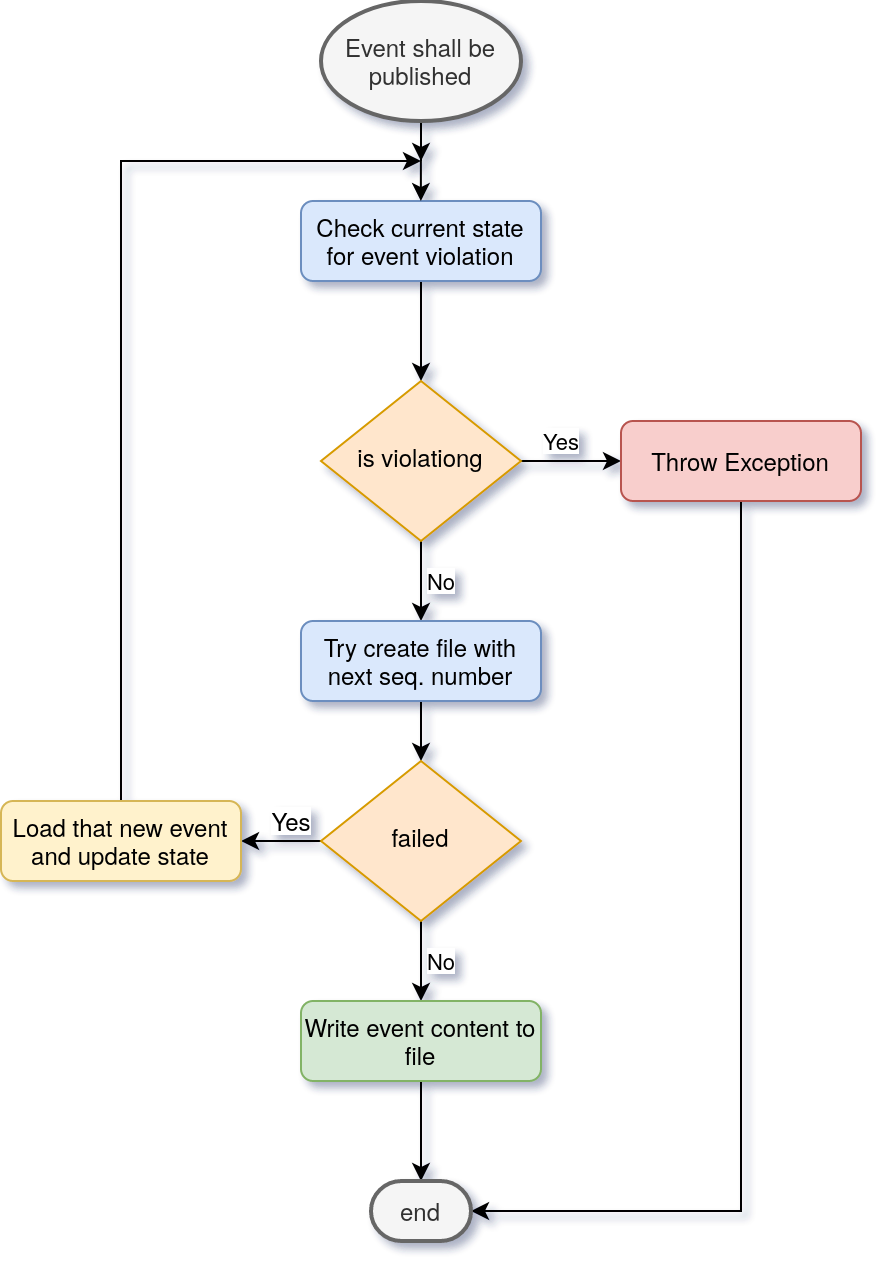
\includegraphics[width=0.65\textwidth]{event_publishing.png}
	\caption{Event publishing process}
	\label{event:synchronized_publish}
\end{figure}

Every Winslow instance is responsible for keeping track of all global states and check before publishing a new event whether the state would be violated by this event.
If it is not, it will try to publish it by creating a new file with the next sequence number.
If the file already exists, another instance did publish an event in the meantime.
This externally published event must then be loaded and the global state updated before a new attempt in publishing the original event can be made.
Eventually, this will either lead to successfully publishing the event or failing due to state violation - for example trying to lock a project that is already locked.


This synchronization mechanism ensures that each event is only published if it is not violating any constraints, such as locking resources that are already locked.
It also allows for multiple locks and elections to happen concurrently, as long as there is no overlap.

\begin{figure}[H]
	\centering
	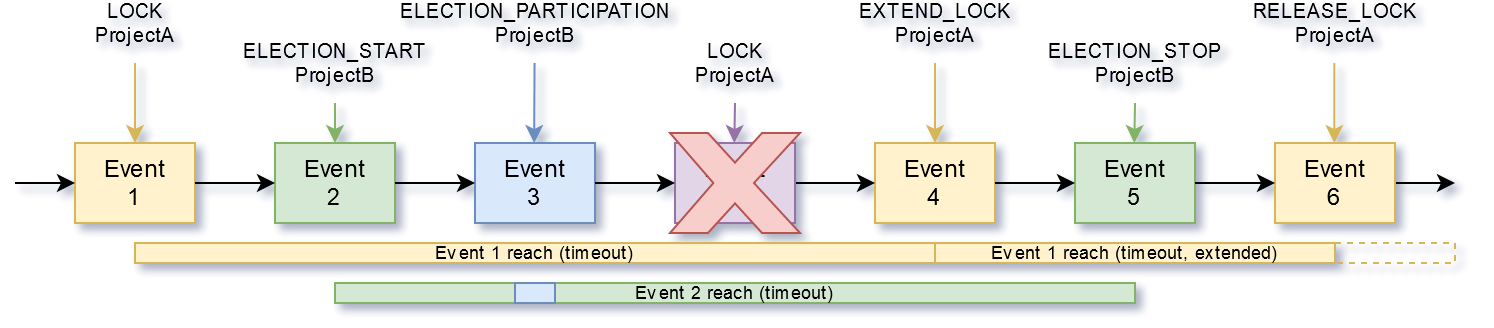
\includegraphics[width=1.0\textwidth]{events.png}
	\label{winslow:com:events}
	\caption{Sample event and lock series with lifetimes}
\end{figure}

In \autoref{winslow:com:events} a series of events, their sequence number and commands are shown.
The coloured rectangles below shows the duration of their lifetimes.
The crossed-out event is violating the constraint that a resource can only be locked by one instance at a time: the yellow lifetime in this case.
Because of this violation the even is never published to the event bus, which is demonstrate with the sequence number of the next event not skipping the number 4.

\section{Docker interface}


To interface with the Docker daemon a driver implementation is needed.
It needs to on container creation commands with a set of environment variables and the path to a prepared workspace.

Docker provides a REST API\cite{docker:api} for third party libraries as well as implementations in Go and Python.
There is no official Java API implementation.
This means, either a third party Java library must be used, the REST calls that are required have to be implemented within this project or another alternative must be found.
The Docker REST API is very expressive which is a reason to not implement the REST calls within this project.

As it turns out, the Nomad Project, which was already investigated in \autoref{nomad}, provides a library with a thin abstraction layer and lots of reasonable default values.
It also includes support to create container that use the Docker plugin from Nvidia\cite{nvidia:docker_plugin}.
This allows attaching GPUs to a container without the need of listing all libraries and device files manually\footnote{If you are interested in how tedious this could otherwise become, see \url{https://github.com/hashicorp/nomad/issues/3499\#issuecomment-364214506}}.
The scheduling capabilities of Nomad are not used because the focus of nomad does only overlap partially with the needs of Winslow.
A job is expected by Nomad to rerun, moved to different hosts and - in the service mode - scaled as it seems needed.
The control of where the job is executed is then lost, which is not acceptable when different firewall rules apply to all Winslow instances and a judgement for the best hardware utilization was already made.
Furthermore, when using GlusterFS or another cloud storage or compute capabilities, the network share is not always reachable through the same proxy for every node.
The lack of control could then cause stage execution failures due to unreachable workspaces.
Nomad will therefore only be used in the local Winslow container as thin layer to interface with an enriched Docker API.

%\todo{because: nomad focuses on scheduling multiple instances of a load balanced service, lack of control on where it is spawned, additional communication channels required -> firewall/admin/maintanance, interfer with further extenstions cloud like cloudstore and GlusteFS because a 'randomly' by nomad chosen node would require access to the storage which might not be visible to all executions nodes through the same path}.


\section{Directory Structure and Organization}

This section describes the organization of the working directory for the Winslow instances.
Because a common network share is required by Winslow for event synchronization and the projects' workspaces, this was further extended to share the configuration and project files as well.
This has the very nice side-effect, that there is no real setup to do when installing a new Winslow instance\footnote{\autoref{appendix:winslow_installation} lists the complete installation script for a new Winslow instance}, it just needs access the to working directory.

For the configuration files, a principle found on Unix and Linux systems was applied: human readable text files.
For complex structures YAML formatting is used, while for simple key value files property formatting is used.
This makes understanding the system state easier when debugging in error scenarios.

\subsection{Winslow working directory}
\label{design:winslow:workdir}

A brief summary of the by all instances shared working directory:

\begin{itemize}
	\item \monospaceinline{logs}: The location for stage log files.
	This includes system events and the console output with timestamps.
	The file name is formatted as \\
	\monospaceinline{<project-id>-<stage-number>-<stage-name>}.
	\item \monospaceinline{pipelines}: Pipeline definition file (YAML) are located here.
	\item \monospaceinline{projects}: Project definition files (YAML) are located here.
	\item \monospaceinline{resources}: The globally available input resources, see \autoref{stage:workspace}.
	\item \monospaceinline{run/events}: The directory used to synchronized events, see \autoref{design:synchronization}.
	\item \monospaceinline{run/nodes}: The directory used to publish node utilization, see \autoref{design:monitor_resources}.
	\item \monospaceinline{settings}: The directory used to share common configurations, currently this only contains a global environment variable configuration.
	\item \monospaceinline{workspaces}: The per project specific workspaces are located here, see \autoref{stage:workspace}.
\end{itemize}

Because the files in \monospaceinline{run/events} and especially \monospaceinline{run/nodes} are very temporary, the NFS server locates these in shared memory (\monospaceinline{/dev/shm}) to reduce stress on IO and unnecessary wear on SSDs.
%Thanks to the synchronization and locking mechanism (presented in \autoref{design:synchronization}), the working directory can shared between all Winslow instances.

\subsection{Stage storage}
\label{stage:workspace}

The storage organization for a project and its stages had a few unexpected concerns raised.
%Thinking about the storage organisation for the pipeline and its stages, a few expectations and concerns arise.
First of all, to redo a stage, one needs to be able to access the files that were the result of one, two or multiple stages before.
Sometimes a stage wants to access intermediate data produces by multiple previous stages.
Next, the input video footage needs to be accessed by multiple stages throughout the pipeline execution.
Finally, some stage results are not intermediate but do already present some final results.

The first and second concern can be solved by providing a workspace directory for each stage, that is copied from the logically previous stage\footnote{the stage the new one is based on, this does not always need to be the numerical previous stage}.
Once the computation of a stage is completed, the workspace is considered immutable and only used to source new workspaces from.
This works fine for small intermediate results, but it does not work very well for large files - like the video footage.
This delays the start of the stage execution, requires unnecessary storage due to multiple copies and provides no benefits in an archival and version control sense, because the video footage is not altered.
So there needs to be another storage pool for input data, that is globally accessible and never changed: the global input storage pool.
Providing one further storage pool for final results (global output pool), concern number three and four are also solved.

Because the very first stage has no workspace to source its files from, on creation of the project a workspace directory for the \enquote{zeroths} stage is created.
The user can then provide the very first stage with a predefined and non-empty workspace if necessary.

This also solves te problem with delays due copy operations in NFS, which are performed client side.
This means, the client reads the input file and writes to the output file\footnote{Server-side copy has just been standardized for NFS 4.2\cite{nfs:ssc}}.
This operation does not only take unnecessary long but also utilizes all available network bandwidth which then cannot be used by other applications.

To ensure that the global input and the previous intermediate results are not altered, the Docker daemon is instructed to mounted them as read-only filesystems.
This also prevents bugs or errors from accidentality deleting unrelated files\footnote{\enquote{This so theoretical and will actually never happen in real life} proven otherwise: \url{https://github.com/valvesoftware/steam-for-linux/issues/3671}}.
\autoref{storage_organization} summaries all this:


\begin{figure}[H]
	\centering
	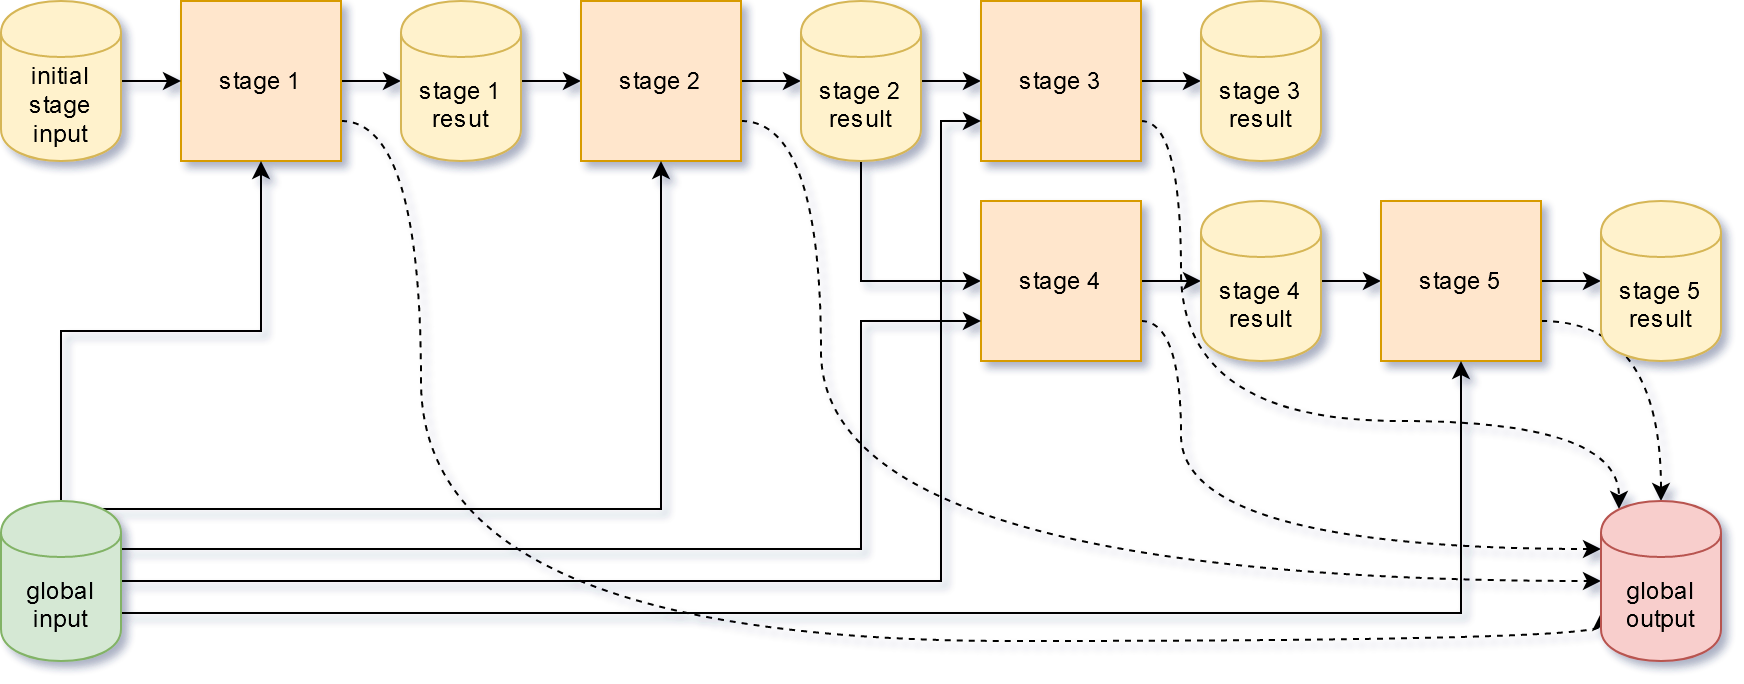
\includegraphics[width=0.9\textwidth]{stage-storage.png}
	\caption{Stages with their intermediate and global resource pools}
	\label{storage_organization}
\end{figure}

For a running stage the mounted directories looks like the following:

\begin{itemize}
	\item \monospaceinline{/input} is mounted read-only from \\ \monospaceinline{nfs-server:/winslow/workspaces/<project-id>/input}
	\item \monospaceinline{/output} is mounted with write permissions from \\ \monospaceinline{nfs-server:/winslow/workspaces/<project-id>/output}
	\item \monospaceinline{/workspace} is mounted with write permissions from \\ \monospaceinline{nfs-server:/winslow/workspaces/<project-id>/<stage-id>} \\
	and was created by the copying the workspace directory of the logically previous stage into it
\end{itemize}


%\todo{define logically previous stage -> previous stage on linear execution and ... when jumping around}
%stage execution does not need to depend on the result of the exact previous



\section{Job Scheduling and Election System}
\label{design:election}

Winslow has no ahead of time plan to schedule stage executions, the main reason for this that it is unknown how long a stage is about to take.
One could consider to build statistics to eventually be able to guess the duration of repeatedly executed stages, but this seems error prone, does not cover seldom executed stages and is in addition unreasonable complex.
%\todo{mention these complex scheduling techniques?}
Instead, the system is reacting to user submissions and on stages that have just completed.
For each new execution, an election is then held in which the winner will execute the stage.
Winslow instances that do not fulfil the resource requirements do not participate in the election.

\subsection{Affinity and Aversion}
\label{election:affinity_and_aversion}

To determine a winner, participants must be comparable.
Winslow uses a two factor scoring mechanism for that, in which it judges how efficient a node is going to be utilized (affinity scoring) and how many unused resources will be wasted (aversion scoring).
The instance with the highest affinity value out of the instances of the lowest aversion values wins.

This system was developed within this thesis but loosely inspired by Nomad\cite{nomad:main}, which also uses an affinity score\cite{nomad:affinity} but no aversion equivalent.
Instead of specifying this value in each job definition like in Nomad, Winslow derives it's values from the available resources and resource requirements.
This requires less user interference, prevents blocking unused hardware and still delivers good results, as will be discussed next.

For determining the affinity scoring only requested resource categories $c_i$ need to be considered.
Through the resource monitoring (see \autoref{design:monitor_resources}) the total resources $r_{c_{max}}$ as well as the reserved resources $r_{c_{in\_use}}$ are known.
For every requested resource by the stage definition $c1 .. cx$, the ratio between requested $r_{c_i}$ and available resources is calculated.
The lowest ratio, and therefore the most pessimistic value, of any category is used as the affinity score:

\begin{equation}
	\label{election:eq:affinity}
	\text{affinity} = \min_{c_1 .. c_x} \left( \frac{r_{c_i}}{r_{c_{max}} - r_{c_{in\_use}}} \cdot n_{c_x} \right)
\end{equation}

As seen above, every node can additionally apply a resource category specific multiplier $n_{c_x}$ for punishment or gratification.
This allows to fine tune the score on a per node basis.

For determining the aversion scoring, all by a node available resource categories $c1 .. c_a$ need to be considered.
In contrast to the affinity score, the highest ratio of any unused resource is used as aversion score, which is again the most pessimistic value.

\begin{equation}
	\label{election:eq:aversion}
	\text{aversion} = \max_{c_1 .. c_a} \left( \frac{r_{c_{max}} - r_{c_{in\_use}} - r_{c_a}}{r_{c_{max}}  - r_{c_{in\_use}}} \cdot n_{c_a} \right)
\end{equation}

The more resources are wasted - especially categories that are untouched at all - the worse the aversion score.

An example shall illustrate the scoring system.
Lets consider the following three execution nodes exist:

\begin{table}[H]
	\centering
	\begin{tabular}{|l|r|r|r|}\hline
		 & Free CPUs & Free memory & Free GPUs \\
		 \hline
		 Node 1 & 4  	& 16 GiB & 0 \\
		 Node 2 & 12 	& 58 GiB & 0 \\
		 Node 3 & 4 	& 50 GiB & 1 \\ \hline
	\end{tabular}
	\caption{Nodes to consider}
\end{table}

The following three stages executions shall be assessed:

\begin{table}[H]
	\centering
	\begin{tabular}{|l|r|r|r|}\hline
		& Req. CPUs & Req. memory & Req. GPUs \\
		\hline
		Ex1 & 2 & 16 GiB & 0 \\
		Ex2 & 4 & 48 GiB & 0 \\
		Ex3 & 4 & 16 GiB & 1 \\ \hline
	\end{tabular}
	\caption{Stage executions to consider}
\end{table}

The following table shows the resulting affinity and aversion score.
The winning node for is marked by the bold formatting.


\begin{table}[H]
	\centering
	\begin{tabular}{|l|r|r|r|}\hline
		& Node 1 & Node 2 & Node 3 \\
		\hline
		Ex1 & \textbf{0.5/0.5}	& 		  0.28/0.72	& 		  0.32/1.0 \\
		Ex2 & - 				& \textbf{0.34/0.67}& 		  0.96/1.0 \\
		Ex3 & - 				& - 				& \textbf{0.32/0.68} \\\hline
	\end{tabular}
	\caption{Affinity/Aversion score for every stage definition and node constellation that provides all required resources}
\end{table}

As shown in the example, the aversion score is important to prevent stages taking execution nodes that provide specialised hardware (such as GPUs) which is not required by the stage execution.
In this example, it prevent Ex2 to be scheduled on Node 3, which provides a GPU.

In comparison to just forbidding executions on nodes with hardware that is not used, in scenarios where all general purpose nodes have failed, are unreachable or stage execution has very little requirements, this system would still schedule executions.
But it tries as best as possible to prevent blocking unused resources, like Ex1 and Ex2 running on GPU nodes.

\section{Execution}

The execution of a stage is started on the Winslow instance that won the corresponding election.
It first locks the project, to re-read the configuration and to prevent any changes to in the meantime.
The workspace is being prepared (see \autoref{stage:workspace}), environment variables collected and the backend driver instructed to start the new container.
Any data logged to the containers' stdout or stderr is collected and written to a log file exclusive to this stage execution (see \autoref{design:winslow:workdir}).
System related events, such as errors pulling an image, exhausted resources or sudden aborts are also logged to this file.

A lock on the project is not held during all the time the stage is being executed, because it would prevent stages being enqueue and or prepared by a user in the meantime.
Instead, after successfully starting the new container and the log file has been created, a new lock pointing to the log file is created.
The currently executed stage is noted in the project file and then the lock on it is released.
As long as the lock for a log file is alive, no election for the project is allowed.

Once the container has stopped - and the stage has therefore either failed or succeeded - the lock on the project is acquired again to update the stage state.
After this, both locks are released, potentially triggering the next election.

\begin{comment}
\todo{affinity}
\todo{aversion}

Utilizing Event Bus for timely limited elections and to ensure that there are no concurrent election for a single project.

\todo{what about concurrent elections on multiple projects}

\todo{regarding locking: check for updatable, try to lock, check for updatable again, update, unlock}

\todo{on unlock: check updatable}



\todo{scheduling / job assignment/pull strategy}

\todo{graph displaying over time lock and election}
\end{comment}


\section{CPU, RAM and IO Monitoring}
\label{design:monitor_resources}

Monitoring the hardware utilization can be accomplished by parsing the contents of \monospaceinline{/proc/cpuinfo}\footnote{\url{https://www.kernel.org/doc/Documentation/cputopology.txt}}, \monospaceinline{/proc/stat}, \monospaceinline{/proc/meminfo}\footnote{\url{https://www.kernel.org/doc/Documentation/vm/hugetlbpage.txt}}, \monospaceinline{/proc/net/dev} and \linebreak\monospaceinline{/proc/diskstats}\footnote{\url{https://www.kernel.org/doc/Documentation/ABI/testing/procfs-diskstats} and \url{https://www.kernel.org/doc/Documentation/iostats.txt}}.
These special files in the \monospaceinline{/proc} directory are text files generated by the Linux kernel to summarize the current utilization\cite{linux:doc:proc}.

Each Winslow instance is repetitively reading and parsing these files and writing a summarized version to the shared workspace directory \monospaceinline{/run/node/<node-name>}.
An summary example can be seen in \autoref{appendix:run_nodes}.

\section{User Interface}
\label{design:springboot}

To display data on the user interface\footnote{Screenshots in \autoref{appendix:screenshots}}, REST requests are sent to the web-backend of Winslow.
To handle these requests and to serialize the responses Spring Boot\cite{springboot} is used by Winslow.

To not stress the event bus with lock requests caused by the user, all data retrieval operation open and read configuration files without locking them.
This bears the risk of reading incompletely written files, but as the user interface is not crucial to the system and as it must account for failed requests due to network issues anyway, this is considered acceptable.
The user interface would simple resubmit its request.
% \todo{ACID hazards ref?}

When modifying settings or triggering stage executions, the request handling must obey the locking rule to not introduce inconsistent state to the system (due to a dirty read\cite[2]{berenson1995a} that could occur without locking).
This means, on a HTTP POST request, the affected resource is being locked, updated and released.
The release will then trigger a Winslow instance to check the file for potentially starting an election.


%\todo{REST request, read only: no lock; for changes: POST -> LOCK -> update -> RELEASE, on RELEASE Winslow gets notified and checks whether the new configuration leads to a new stage execution}




\begin{comment}
\section{File system}

\todo{docker can auto mount nfs to container}

\subsection{Every node has a connection to every other node}

\subsection{Centralized broker}

\subsection{Tree hierarchy}

\subsection{outcome}




\section{Communication and Node Management}

The system that shall be developed, is supposed to spread jobs onto execution nodes as available.
There are two main approaches in nod management and job assignment.



\subsection{Centralized Management, Remote Execution}

In the central management approach, there is always exactly one leader at any given moment in time.
It is the responsibility of this leader to decide what to execute and where to execute it.

\subsection{Decentralized Management, Local Execution}

\subsection{Combinations worth noting}

stupid:
 - centralized management, local execution
 - decentralized management, remote execution
 
combination, decentralized + some remote slaves

\subsection{Architecture}

event based

common file system for communication because minimum requirements

stick to unix principles(list): simple, human readable intermediate format

voting/election by capabilities and 'will' of a node to run a stage

\todo{providing live hw utilization}

\todo{the whole properties thingy}

\subsection{Failure handling}
\todo{handling failed stages}

\todo{handling failed nodes}

\section{Communication/Event architecture?}

\section{Targeting capabilities}

\subsection{General thoughts}

\section{Planned}

\section{Implementation details}

\section{Synchronization, Locking, publishing events}

\section{REST for UI}



\subsection{Atomicy of (Unix) Filesystems}

\subsection{Atomicy and behavior of NFS in particular}

\subsection{Using as lock backend}

\subsection{Using as election backend}
\end{comment}




%\section{Agile development}

%\todo{.depends, maybe to shallow and not worth noting, dont forget to then ref to \autoref{fundamental:agile}}


\section{Continuous Deployment}

Winslow uses GitLab CI to continuously deliver runnable Docker Images after each git push.
Every code change triggers a new build pipeline, that builds and tests Winslow, packages all dependencies\footnote{Nomad and the Angular Web-Application} into a Docker image and pushes it to our in house private Docker Registry.
Broken code or failing unit tests will result in a notification for the developer and prevents the image from being published.

To update an execution node, the Docker container can simple be stopped and discarded.
The installation script\footnote{Which is displayed in \autoref{appendix:winslow_installation}} then pulls and starts the most recent image.